\chapter{Analyse} \label{anlayse_capter}

In diesem Kapitel wird der Stand der Forschung zu Themen welche für diese Arbeit eine hohe Relevanz darstellen behandelt. Dazu zählen wie Annotationen in virtuellen Umgebungen, das Zeigen und Auswählen in AR sowie die Kundeniteration mit immersiven Methoden.

\begin{comment}
\section{Augmented Reality Frameworks}

In diesem Abschnitt wird eine Übersicht über Augmented Reality Framework nach aktuellem Stand der Technik gegeben.

%ARKit ARCore SLAM!
Zum aktuellen Stand der Technik 

%Vuforia, Wikitude... Marker, Natural Feature, 3dObject

%Visionlib 3D Objekt spezialisiert. 

%Unterschide 3D Objekt basiert Vuforia und visionlib: Vuforia - keine Objekte mit geringer geometrischen eigenschaften. Vuforia, bewegungsempfindlich. 

%Vuforia kann mit ARCore oder ARKit kombiniert werden!
\end{comment}

\section{Informationsdarstellung in virtuellen Umgebungen}\label{brand_abschnitt}

Mit Anwendung des digitalen Prototypen sollen Feedback in Form von Annotationen auf dem physischen Produkt dargestellt werden. 
In diesem Abschnitt werden Forschungen zu Annotationen in Virtuellen Umgebungen insbesondere der Usability-Aspekte dieser Darstellungsform näher betrachtet. 

\citeauthor{Brandenburg2019} befasst sich in ihrer Arbeit mit unterschiedlichen Informationsdarstellungsformen in virtuellen Umgebungen.
Sie vergleicht hierbei in einer Studie zwei unterschiedliche Darstellungsformen in einer CAVE \footnote{CAVE kurz für \textit{Cave Automatic Virtual Environment}, bezeichnet einen Raum in welcher drei bis 6 Wände Projektionsflächen sind und dem Nutzer durch das Tragen von Schutterbrillen ein Eindruck von ... erscheint } hinsichtlich Usability-Aspekte für virtuelle Design-Review Prozesse in der virtuellen Produktentstehung. Dabei wird ein besonderer Fokus auf die Art der Aufgabe der Review-Teilnehmer gelegt.
\cite[S.~48]{Brandenburg2019}

Bei einer virtuellen Design-Review wird das 3D-Modelle eines Produktes bzw. verschiedene Ausführungen davon von einem interdisziplinären Reviewteam betrachtet um Entscheidungen zu treffen. 
Herbei werden neben dem 3D-Modell des Produktes Informationen zum Produkt bzw. zu den einzelnen Produktteilen betrachtet welche für die Entscheidungsfindung relevant sind. \cite[S.~32]{Brandenburg2019}
 
In Anlehnung an \cite{Polys2004} \cite{Polys2007} identifiziert \citeauthor{Brandenburg2019} zwei unterschiedliche Aufgabentypen welche einen Einfluss auf die jeweiligen Darstellungsformen haben: Such und Vergleichsaufgaben. 
Eine Suchaufgabe kann dabei z. B. folgende Frage sein: ``Wo ist der Motor?`` eine Vergleichsaufgabe hingegen: ``Was befindet sich im Kofferraum und wie wird es bezeichnet?``. \cite[S.~52]{Brandenburg2019}

Annotationen welche nicht direkt am betreffenden Produktteil dargestellt werden sondern um das Produkt herum auf einer eigenen Ebene, führen zu mehr Genauigkeit, weniger Bearbeitungszeit und erhöhter Zufriedenheit bei der Lösung einer Suchaufgaben. Dies begründet sich dadurch dass Annotationen in dieser Anordnung nicht überdecken. Wogegen Annotationen welche direkt an den betreffenden Produktteile dargestellt werden, sich besser für Vergleichsaufgaben eignen. Dies begründet sich dadurch dass bei diesen Aufgaben eine Übertragungsleistung von bildlichen zur textuellen Information nötig ist. \cite[S.~52]{Brandenburg2019} 

In der Studie wurde neben der getrennten Darstellung von Text und Produktteil, als eine weitere unabhängige Variable die Darstellung mit oder ohne Verbindungslinie welches Annotation mit dem Produktteil 
verbindet betrachtet. Abbildung \ref{img:uv} zeigt die evaluierten Darstellungsformen.

\begin{figure}[H]
	\centering 
	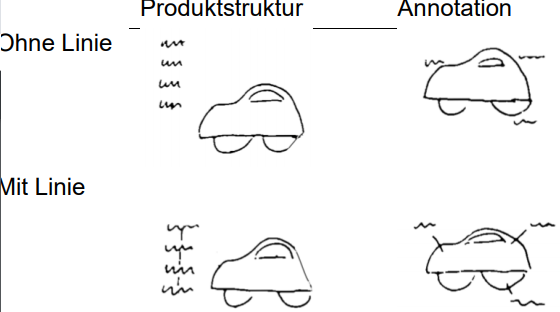
\includegraphics[width=.6\textwidth]{resources/analyse/brandenburg_uv.png}
	\caption{Darstellungsformen welche in der Studie evaluiert wurden. Quelle: \cite[S.~127]{Brandenburg2019}}
	\label{img:uv}
\end{figure}

Auf Abbildung 3.2 linke Seite, ist die getrennte Darstellung als Baumstruktur zu sehen. Die einzelnen Bauteile sind mit Verbindungslinien an Elternknoten welche eine Baugruppe bilden verbunden dargestellt. In der Studie wurde jeweils ein Begriff aus der Baumstruktur sowie ein Produktteil am Auto farblich grün hervorgehoben. 

Abbildung 3.2 rechte Seite, zeigt die Darstellung als Annotation. Hier wurde die Begriffe welche zu einer Baugruppe gehören durch eine grüne Einrahmung der jeweiligen Annotation von den anderen 
Annotationen farblich hervorgehoben.  

\begin{figure}[H]
	\centering
	\begin{minipage}{.5\textwidth}
		\centering
		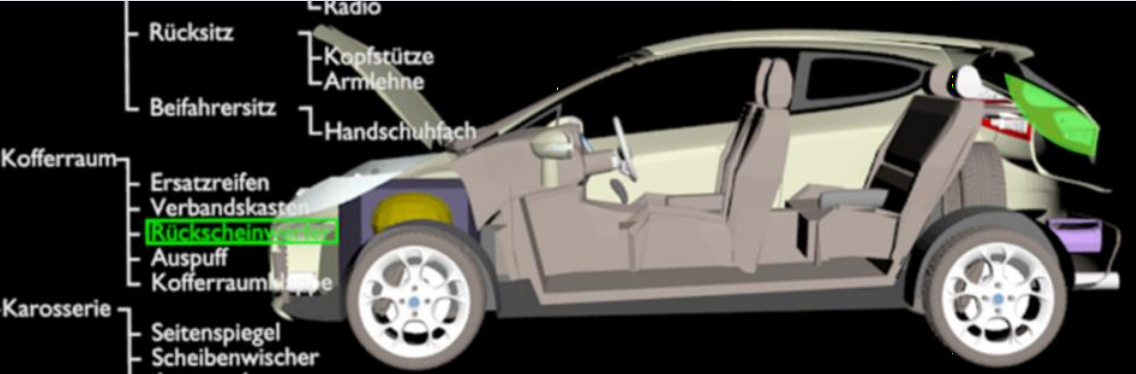
\includegraphics[width=.95\linewidth]{resources/analyse/baumstruktur.png}
		\label{fig:baum}
	\end{minipage}%
	\begin{minipage}{.5\textwidth}
		\centering
		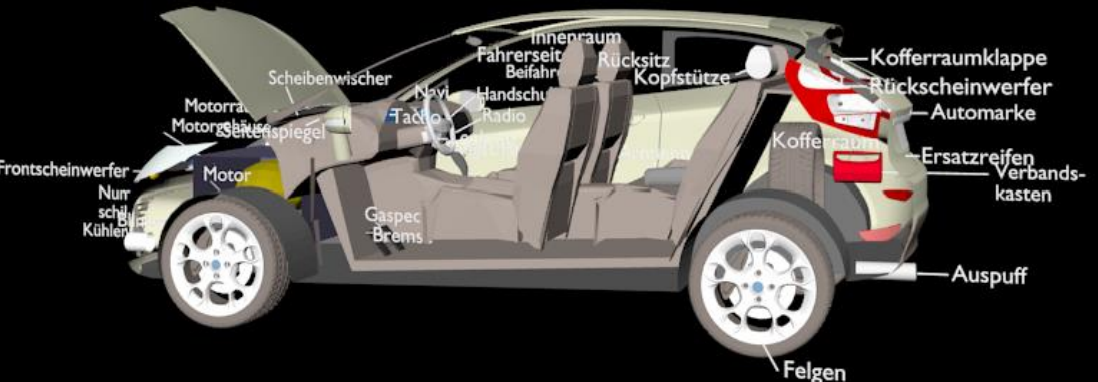
\includegraphics[width=.95\linewidth]{resources/analyse/annotation.png}
		\label{fig:annotation}
	\end{minipage}
\caption{Unterschiedliche Darstellungsformen - Links: Darstellung als Baumstruktur getrennt vom Produkt. Quelle: \cite[S.~127]{Brandenburg2019} Rechts: Darstellung als Annotation, am jeweiligen Produktteil. Quelle: \cite[S.~128]{Brandenburg2019}}
\label{img:versuchAbbildung}
\end{figure}

Abbildung \ref{img:aufgabenbeschreibung} zeigt die Aufgabenstellungen welche von den Versuchspersonen gelöst werden mussten:

\begin{figure}[H]
	\centering 
	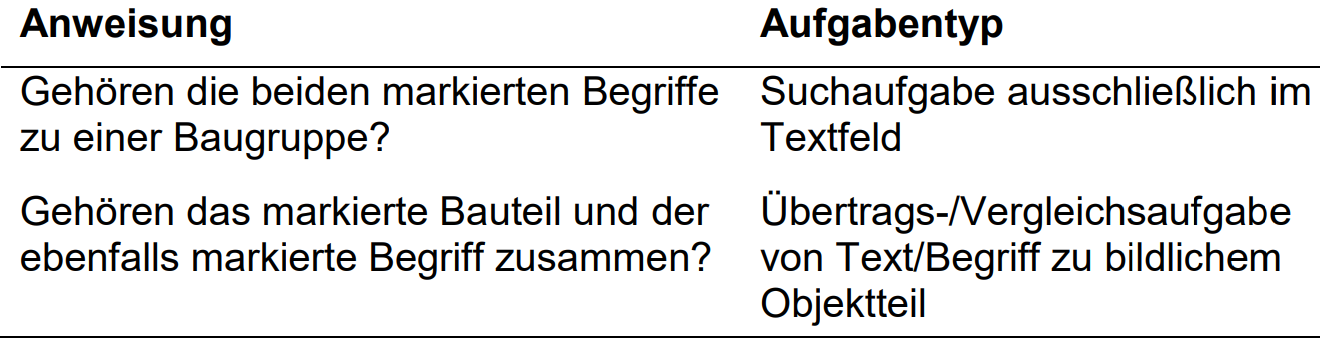
\includegraphics[width=.6\textwidth]{resources/analyse/brandenburg_aufgabentypen.png}
	\caption{Aufgabenbeschreibungen - Suche und Vergleichsaufgaben. Quelle: \cite[S.~132]{Brandenburg2019}}
	\label{img:aufgabenbeschreibung}
\end{figure}

Im Ergebnis dieser Studie konnten die Effekte beider Darstellungsformen auf die jeweiligen Aufgabentypen haben, welche von \citeauthor{Polys2007} in \cite{Polys2007} beschreiben werden, bestätigt werden.
Des weiteren hat sich in dieser Studie herausgestellt dass Annotationen welche mit einer Verbindungslinie dargestellt werden welches Text mit entsprechendem Produktteil verbindet 
zur effizienteren Lösung der Aufgabe beitragen.Quelle: \cite[S.~135]{Brandenburg2019}

\section{Zeigen und Auswählen in AR Benutzeroberflächen} \label{pointer_section}

In diesem Abschnitt werden Grundlagen für das zeigen und Auswählen in Virtuellen Umgebungen behandelt, sowie einige aktuelle Arbeiten 
zu diesem Thema näher betrachtet. 

Der digitale Prototyp soll auf ein Touchscreen Bildschirmoberfläche eines Smartphones genutzt werden.
\citeauthor{Ortega2016} beschreiben folgende grundlegende Probleme welche bei Interaktionen auf diesen Oberflächen auftreten können und daher beachtet werden sollten:  
Dadurch dass Interaktionen mit dem direkten Berühren des Bildschirmes stattfinden fehlt bei Touch Oberflächen das Drüber schweben (engl. Hover) bevor eine Aktion durch das Klicken der Maus Taste bestätigt wird. 
Dadurch dass der Finger auf den Bildschirm aufgelegt wird, besteht das Problem der Verdeckung. Zudem muss mit stark variierender Sinn für Präzision gerechnet werden. Weiter ordnen \cite[S.~205]{Ortega2016} Ansätze 
für die Behandlung dieser Probleme in zwei Gruppen ein: Die erste Gruppe behandelt diese Probleme in der Gestaltung der Benutzeroberfläche. Während in der zweiten Gruppe für die Lösung dieser Probleme, die Intension 
der Nutzers untersucht wird und die Interaktion entsprechend ausgeführt wird. \cite[S.~205]{Ortega2016}

Die Aufgabe ein Objekten in virtuellen Umgebungen auszuwählen, setzt sich aus einer Komposition dreier Teilaufgaben zusammen welche jeweils unterschiedlich umgesetzt werden können. 
Diese Teilaufgaben werden in \cite[S.~12]{Bowman1999} \cite[S.~150]{Bowman2011} als folgende vorgestellt: 

\begin{itemize}
\item \textit{Andeutung der Selektion eines Objektes (engl. Indication of object).} Dem Nutzer wird die Möglichkeit gegeben auf ein Objekt oder auf ein Bereich zu zeigen welches ausgewählt werden soll.
\item \textit{Bestätigen der Auswahl (engl. Confirmation of selection bzw. Indication to select).} Es werden Techniken zur Verfügung gestellt womit der Nutzer sein Auswahl bestätigen kann. 
\item \textit{Rückmeldung (engl. Feedback).} Die Bestätigung der Auswahl wird vom System bestätigt. 
\end{itemize}

Abbildung \ref{img:auswahluebersicht} stellt diese Teilaufgaben in einer Übersicht dar und zeigt einige Beispiele wie diese auf unterschiedlicher weise umgesetzt werden können. 

\begin{figure}[H]
	\centering 
	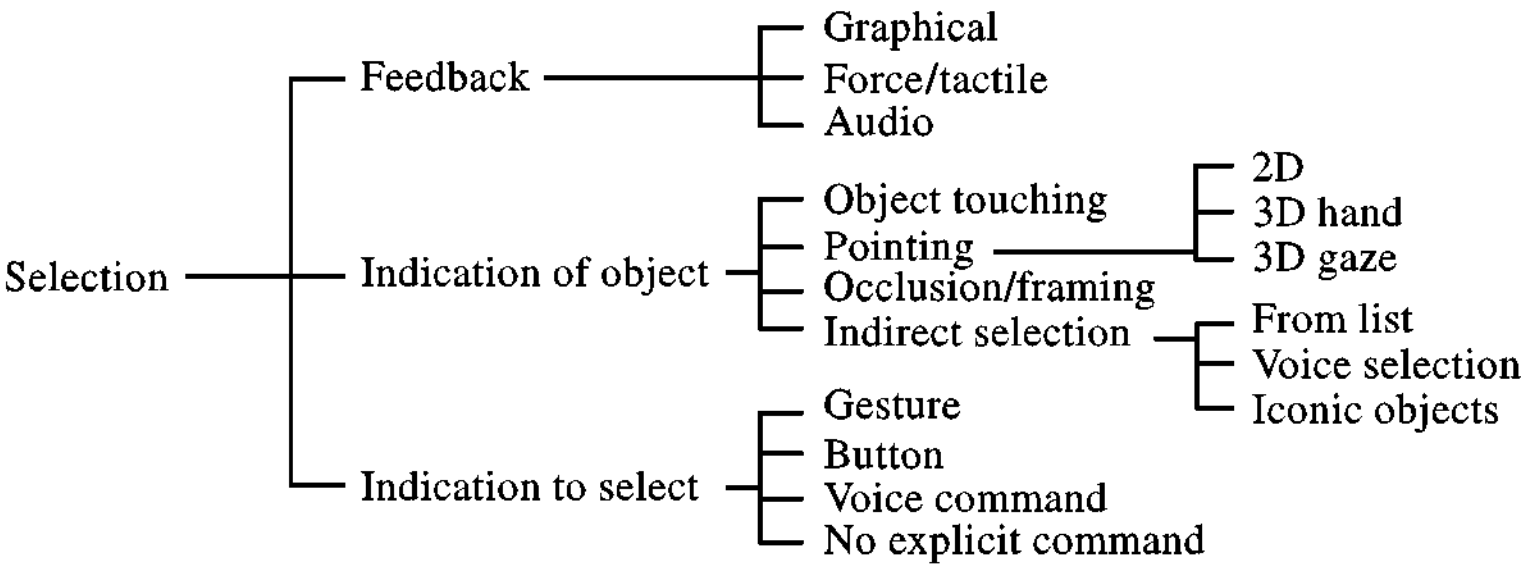
\includegraphics[width=.8\textwidth]{resources/analyse/Selection_uebersicht.png}
	\caption{Klassifikation von Auswahltechniken. Quelle: \cite[S.~12]{Bowman1999}}
	\label{img:auswahluebersicht}
\end{figure}

Beispielsweise kann das Andeuten einer Selektion durch die Auswahl in einer Listenansicht, durch Sprachbefehle oder durch das Zeigen umgesetzt werden. 
Ein Technik für das Zeigen stellt das Ray-Casting dar. Mit dieser Technik wird ausgehend von einer Startposition, in eine Richtung in welche gezeigt wird, ein Strahl 
ausgesendet welches Objekte in der Umgebung treffen kann. Dabei werden Schnittpunkte dieser Strahl mit Objekten aus der Umgebung verglichen und das Objekt    

\citeauthor{Bowman2011} bezeichnet das Zeigen durch Ray-Casting als eines der einfachsten und effektivsten Techniken für das Auswählen in virtuellen Umgebungen für Anwendungsfälle in welchen auf Objekte aus 
naher Distanz gezeigt wird.\cite[S.~153]{Bowman2011}

\citeauthor{Vincent2013} vergleichen in eine Studie zwei unterschiedliche Ansätze für das Zeigen zum Auswählen von Stellen auf planaren Oberflächen. 
Die Studie vergleicht folgende zwei Ansätze mit Anwendung auf zwei unterschiedlichen mobilen Endgeräten - Einem Tablet und einem Smartphone: 

\begin{itemize}
\item{Das Zeigen durch eine in der Mitte des Bildschirm fixierten Fadenkreuzes, diesen Ansatz bezeichnen \citeauthor{Vincent2013} als \textit{Crosshair}. Bei dieser Methode 
befindet sich auf der Mitte des Bildschirmes ein Fadenkreuz. Ausgehend von dieser Stelle wird von der Anwendung ein Strahl in die Umgebung ausgesendet und 
kann Objekte in der Umgebung treffen. Der Nutzer kann auf bestimmte Stellen auf planaren Oberflächen zeigen indem er das Mobile Endgerät bewegt und mit dem Fadenkreuz
auf die Stelle anvisiert (Abbildung \ref{img:pointing_vergleich} (B).} 
\item{Bei der zweiten Methode hingegen, welches als \textit{Relative Pointing} bezeichnet wird, wird der Fadenkreuz auf die Oberfläche fixiert, auf welchem die Selektion stattfinden soll. Der Nutzer kann die Position des Fadenkreuzes durch das Wischen auf der 
	Touchscreen Oberfläche verändern (Abbildung \ref{img:pointing_vergleich} (C).}
\end{itemize}

Zusätzlich wird der Versuch mit dem Zufügen einer künstlich erzeugtem Registrierungs-jitter d. h. einer stark schwankenden Positionsänderung der virtuellen Objekte (Abbildung \ref{img:pointing_vergleich} (D)) wiederholt. 

\begin{figure}[H]
	\centering
	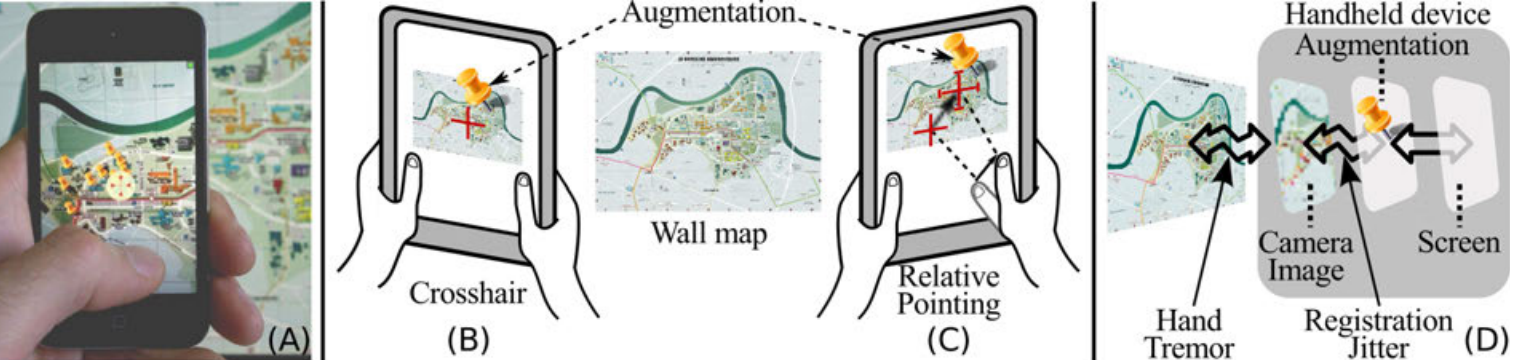
\includegraphics[width=.7\textwidth]{resources/analyse/Pointing_techniken.png}
	\caption{Darstellung zweier Ansätze für das Zeigen und Auswahl auf ebenen Oberflächen. Quelle: \cite{Vincent2013}}
	\label{img:pointing_vergleich}
\end{figure}

An der Studie nahmen 24 Versuchsteilnehmer teil und als Aufgabe musste auf einer Oberfläche, auf welchem kreise, welche ringförmig angeordnet sind ausgewählt werden. Die Kreise 
welche ausgewählt werden sollten sind jeweils blau hervorgehoben worden. Die Teilenehmer haben den Versuch von einer Entfernung aus ca. einem Meter Abstand ausgeführt. 

\begin{figure}[H]
	\centering
	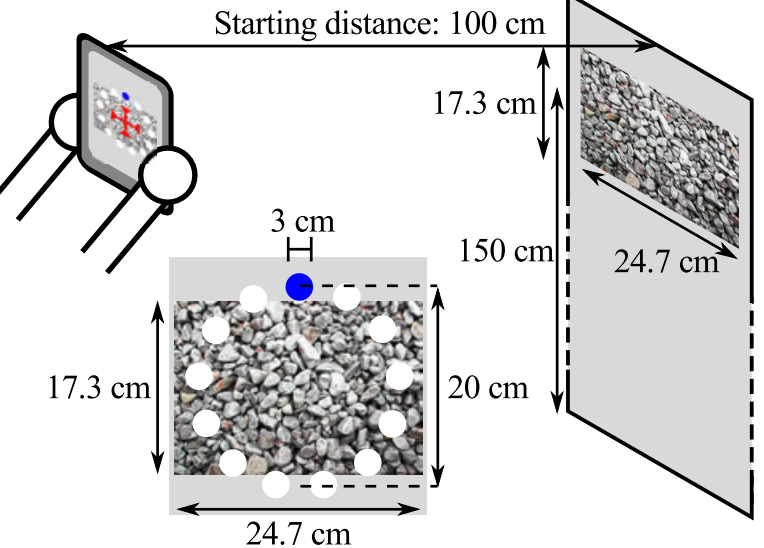
\includegraphics[width=.5\textwidth]{resources/analyse/versuchsaufbau.png}
	\caption{Versuchsaufbau - Vergleich Crossfade vs. Relative Pointing Quelle: \cite{Vincent2013}}
	\label{img:versuchsaufbau}
\end{figure}

Im Fazit dieser Studie kamen bei dieser Studie folgende Erkenntnissen: 

\begin{itemize}
\item{Der Ansatz \textit{Relativ Pointing} führt zu weniger Fehler (Verfehlen der Stelle welche ausgewählt werden soll).}
\item{Zusätzlicher Registirerungs-jitter beeinträchtigt die Genauigkeit der Auswahl mit \textit{Relativ Pointing} geringer.}
\item{Mit \textit{Relativ Pointing} zeigt sich ein geringer Unterschied hinsichtlich Genauigkeit und Dauer des Auswahlvorgangs und der verwendeten Endgerätes. Hingegen zeigt sich bei \textit{Crosshair} ein signifikanter Unterschied in welchem die Performance in beiden Punkten mit der Nutzung des Smartphones schlechter abschneidet.}
\end{itemize}

In einer weiteren Arbeit befasst sich \citeauthor{Vincent2014} mit dem Zeigen auf Oberflächen von drei dimensionalen Objekten. \cite[S.~92]{Vincent2014}

\begin{figure}[H]
	\centering
	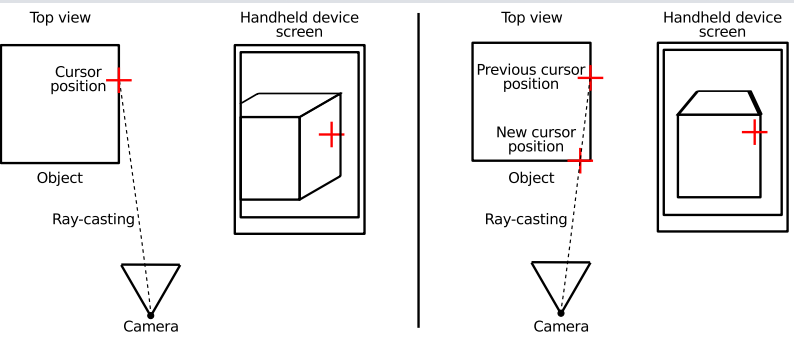
\includegraphics[width=.7\textwidth]{resources/analyse/pointing_3d.png}
	\caption{Relative Pointing auf der Oberfläche von 3D Objekten. Quelle: \cite[S.~84]{Vincent2014}}
	\label{img:pointing_auf3d}
\end{figure}

Bei der Anwendung des \textit{Relative Pointing} auf 3D Oberflächen macht \citeauthor{Vincent2014} auf einen Unterschied aufmerksam: Der Fadenkreuz bzw. der Zeiger kann durch die Struktur des
3D Objektes verdeckt werden oder durch ein Perspektivenwechsel der Kamera, sich nicht mehr im Sichtbereich befinden. Er schlägt für die Behandlung dieses Problems vor, mit Ray-Casting zu überprüfen, 
ob der Zeiger sich im nächsten Schnittpunkt des Ray-Cast befindet und ihn dort zu platzieren falls dieser an einem anderen Bereich befindet. Der Ray-Cast soll dabei ein virtuellen 3D Modell des Objektes treffen.
Als eine alternative dazu schlägt er vor, die Tiefen-Sensor der Kamera zu nutzen diesen Vorgang auf dem physischen Objekt durchzuführen zu können. \cite[S.~83]{Vincent2014}

\section{Immersive Product Improvement (IPI)} \label{ipi_section}

In diesem Abschnitt wird ein von \citeauthor{Kirschner2012} in \cite{Kirschner2012} vorgestellter methodischer Lösungsansatz für Open Innovation (zu dt. Offene Innovation) betrachtet und 
drei unterschiedliche Umsetzungsmöglichkeiten welche \citeauthor{Kirschner2012} vorstellt. 

Open Innovation beschreibt den Innovationsprozess eines Unternehmens, bei welcher interne sowie externe Ideen genutzt werden um diese in der Produktentwicklung umzusetzen und ihr Wissen weiterzuentwickeln. 
Im Gegensatz dazu gehen Impulse zur Innovation in Closed Innovation  lediglich von innerhalb des Unternehmens aus.\cite[S.~32]{Kirschner2012}

Die von \citeauthor{Kirschner2012} vorgestellte Methode setzt ein bereits existierendes Produkt voraus an welchem,  Nutzern,  Nutzungserfahrung sammeln und Verbesserungsbedarf feststellen. 
Diese sollen Nutzer dann als Verbesserungsvorschläge in Form von Kommentaren auf den Produkten, an den entsprechenden stellen anbringen können. Diese Verbesserungsvorschläge sollen dem Hersteller
bei der Überarbeitung der Produkte im Zuge der Modellpflege oder Nachfolgerplanung helfen. Abbildung \ref{img:ipimethode} veranschaulicht diese Methode. \cite[S.~122]{Kirschner2012}

\begin{figure}[H]
	\centering
	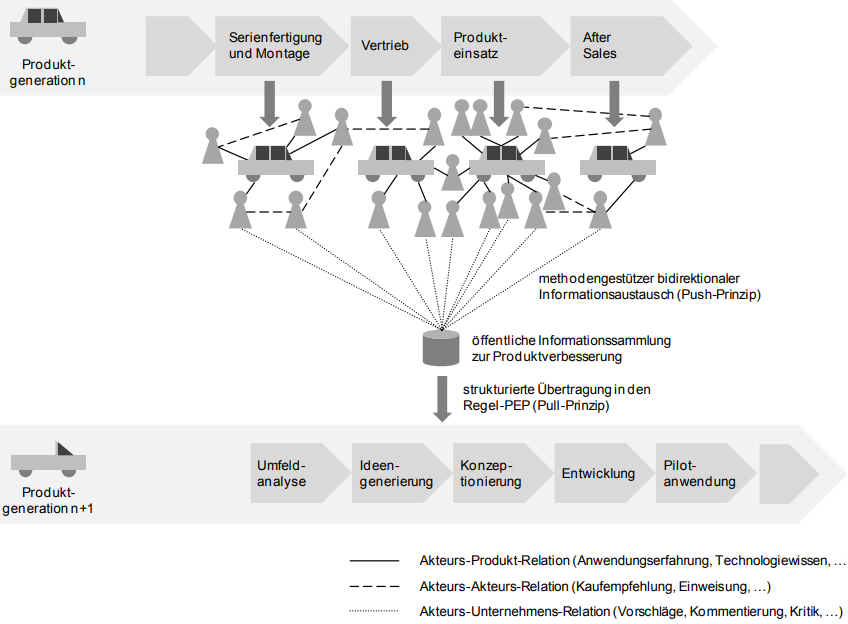
\includegraphics[width=1.0\textwidth]{resources/analyse/IPI_methode.png}
	\caption{Grobkonzept der IPI-Methode. Quelle:\cite[S.~128]{Kirschner2012}}
	\label{img:ipimethode}
\end{figure}

Als Tools für die Umsetzung dieser Methode stellt \citeauthor{Kirschner2012} drei Ansätze vor: Die pysische Umsetzung, bildzentrierten Umsetzung oder objektzentrierten Umsetzung (mit Augmented Reality). 

Mit der phyischen Umsetzung wird ein Exemplar des Produktes ausgestellt und Nutzer können Verbesserungsvorschläge durch das Anbringen von Notizzetteln auf dem Produkt abgeben. 
Dabei sollte nach \citeauthor{Kirschner2012}, darauf geachtet werden dass Notizzettel an Referenzpunkten (an der Stelle am Produkt welche mit dem Beitrag verknüpft ist) angebracht werden. Damit 
soll verhindert werden dass keine gleichen Beiträge für die gleiche Stelle am Produkt abgegeben werden. 

Die Vorteile dieser Umsetzung führt \citeauthor{Kirschner2012} auf, dass diese Methode den höchsten Grad an Immersion bietet, da ein einziges Produkt als  Nutzungs- und
Beitragsbasis verwendet wird. Zudem ist diese Methode kostengünstig und schnell einsetzbar und erfordert keine Serienproduktion. 
Die Nachteile dieser Umsetzung sind jedoch: Einschränkte Anzahl an teilnehmenden Nutzern sowie der Verzicht auf akteursinitiierte Teilnahme, eingeschränkte Skalierbarkeit und aufwendigere Auswertung mit potenziell 
höherer Fehlerquellen. Zudem wäre diese Methode bei länger laufender Einsatz personal bedingt überproportional teuer. \cite[S.~125]{Kirschner2012}

Beim bildzentrierten Ansatz werden Abbildungen des Produktes über eine Onlineplattform des Herstellers zur Verfügung gestellt. Die Nutzer haben die Möglichkeit auf über einer Listenansicht oder direkt auf der 
Abbildung des Produktes bestimmte Referenzpunkte auszuwählen und ein Kommentar dazu abzugeben. Bestehende Kommentare andere Nutzer einsehen und bewertet werden. Weiter können Nutzer bei Abgabe eines Kommentars
diesen thematisch zu einem vom Hersteller vorgegeben Kategorie einordnen. \cite[S.~127]{Kirschner2012}

Zu diesem Ansatz wurde \citeyear{Kirschner2011} von \citeauthor{Kirschner2011} eine Studie durchgeführt worin der Zugang zu Referenzpunkten am Produkt über Listen und Bildansicht verglichen wurde. Abbildung 
\ref{img:ipi_list_image} zeigt beide Ansichten. \cite{Kirschner2011}.

Die Studie wurde mit 48 Teilnehmern durchgeführt wobei die 24 Zugang mit Zugang über die Listenansicht Kommentare abgeben konnten und die anderen Teilnehmer über die Bildzugang. Die Teilnehmer hatten sieben Tage 
Zugang auf die Plattform um Kommentare abzugeben und bestehende Kommentare zu bewerten. 

\begin{figure}[H]
	\centering
	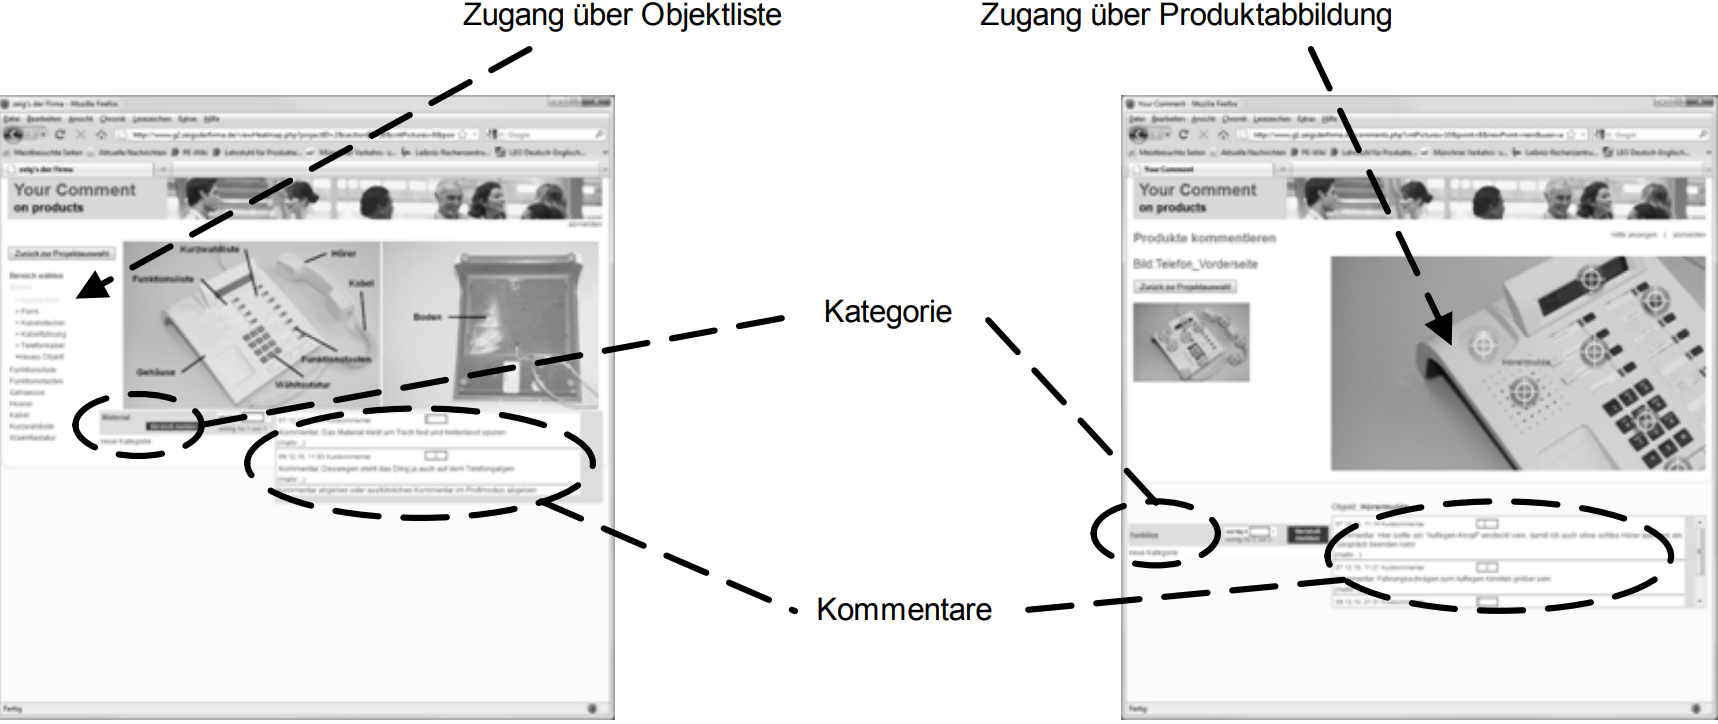
\includegraphics[width=1.0\textwidth]{resources/analyse/IPI_Vergleich_Listen_BildAnnotationeAnsicht.png}
	\caption{Online-Produktkommentierung über Listen- und Bildzugang. Quelle: \cite[S.~7]{Kirschner2011}}
	\label{img:ipi_list_image}
\end{figure}

Im Ergebnis dieser Studie kam heraus dass über Bildzugang deutlich mehr Kommentare erstellt werden gegenüber dem Zugang ober Listenansicht. Auch die Anzahl an Bewertungen (auf Abbildung \ref{img:ergebnisse_listen_bildzugang} sind diese mit ``threads`` bezeichnet) ist ein deutlicher Unterschied zu erkennen. Die Autoren vermuten dass dieser deutliche Unterschied durch die 
zusätzliche kognitive Beanspruchung verbunden ist, die benötigt wird um die textuelle Information aus der Liste mit den entsprechenden Stellen des Produktes zu verbinden.

\begin{figure}[H]
	\centering
	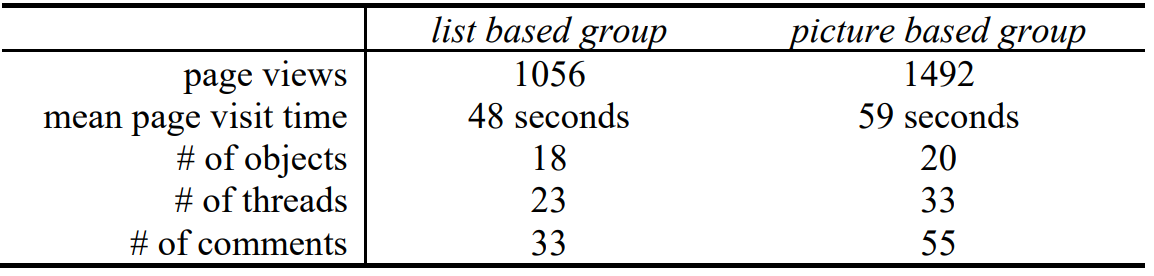
\includegraphics[width=.8\textwidth]{resources/analyse/results_list_picture_based.png}
	\caption{Ergebnisse der Erhebung - Vergleich Liste vs. Bildzugang. Quelle: \cite[S.~7]{Kirschner2011}}
	\label{img:ergebnisse_listen_bildzugang}
\end{figure}

Mit der objektzentrierten Ansatz sollen Nutzer die Möglichkeit haben über die Nutzung eines mobilen Endgerätes das Produkt zu betrachten. 
Durch entsprechende Objekterkennungsmechanismen das Produkt erkannt und bestehende Kommentare auf dem Produkt an entsprechenden Stellen dargestellt werden können.
Dies erfordere die Umsetzung mit Augmented Reality.\cite[S.~135]{Kirschner2012}

\begin{figure}[H]
	\centering
	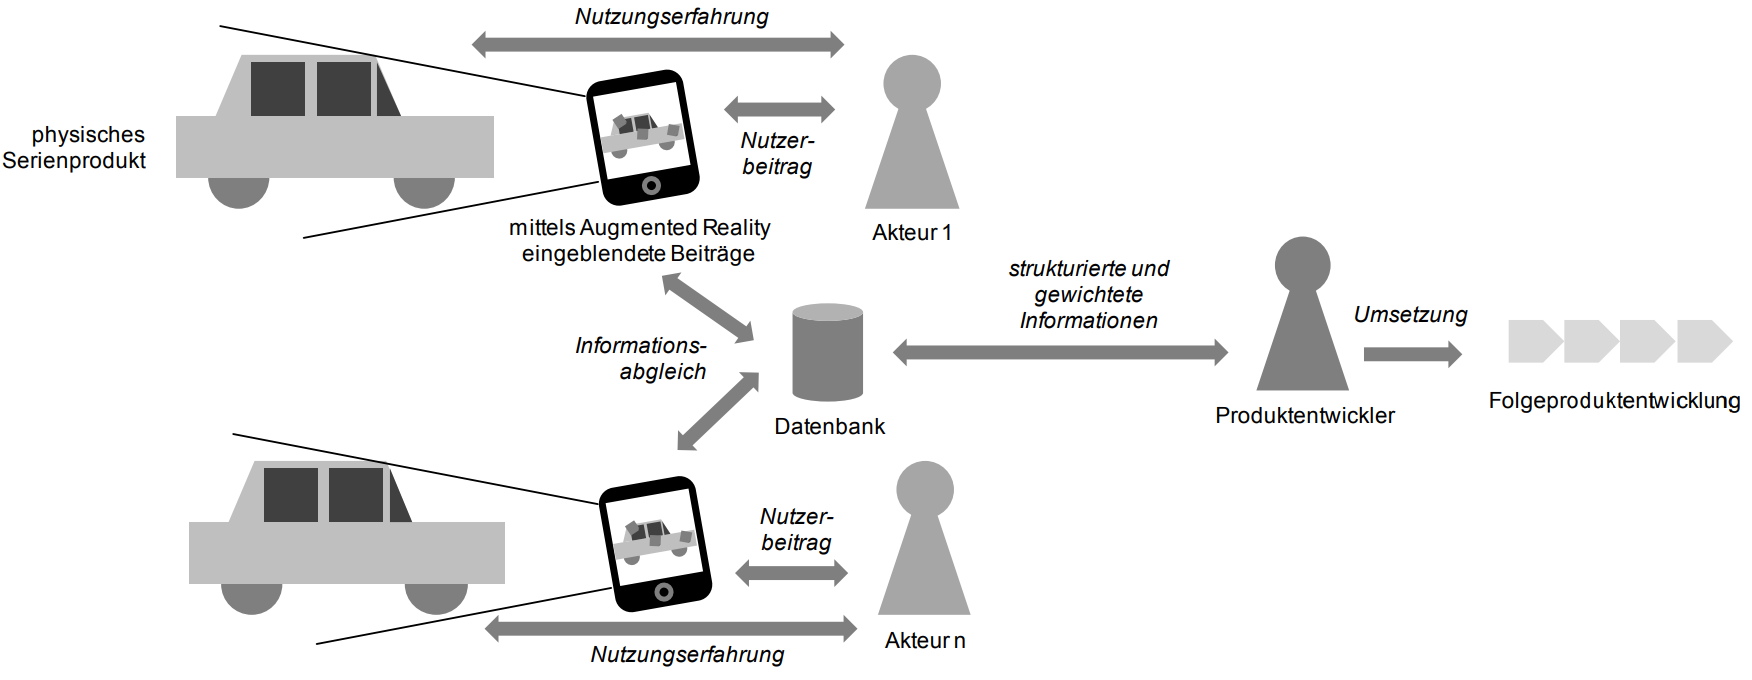
\includegraphics[width=1.0\textwidth]{resources/analyse/IPI_Objektzentriert.png}
	\caption{Informationsfluss in der objektzentrierten IPI-Umsetzung. Quelle:\cite[S.~135]{Kirschner2012}}
	\label{img:objekt_centered_ipi}
\end{figure}

Als Vorteile diesen Ansatzes beschreibt \citeauthor{Kirschner2012}: Dass das Produkt automatisch erkannt werden kann und er Nutzer das Produktbild nicht auswählen muss. Zudem biete dieser Ansatz im Vergleich zum 
bildzentrierten Ansatz einen höheren Grand an Immersion. Als Nachteile beschreibt er dass ein erhöhter Maß an technischen Aufwand für die Umsetzung erforderlich sei und zum aktuellen Stand der Technik die 
Stabilität der technischen Umsetzung noch nicht gewährleistet sei. Weiter beschreibt er dass das Produkt physisch oder zumindest visuell sich vor dem Nutzer befinden müsse und somit ein Teil der Beiträge wegfallen würde.\cite[S.~130]{Kirschner2012}








